\documentclass{beamer}
\usetheme{metropolis}
%\usecolortheme{yellow}

% balíčky

\usepackage[czech]{babel}
\usepackage[utf8]{inputenc}
\usepackage[IL2]{fontenc}

\usepackage{graphicx}

\bibliographystyle{czplain}
\usepackage{balance}

\usepackage{blindtext}
\usepackage{hyperref}

\usepackage{graphics}
\usepackage{picture}
\usepackage{epsf}
\usepackage{epstopdf}
\usepackage{pdflscape}

\usepackage[ruled,vlined,czech,linesnumbered,noline,longend]{algorithm2e}
\usepackage{algorithmic}
\usepackage{listings}

\usepackage{amsmath, amsthm, amssymb, amsfonts, bm}
\usepackage{mathtools}

% informace o dokumentu

\title[]{ITY -- 5. projekt}
\subtitle[]{QuickSort}
\author{Mušková Kateřina}
\date{\today}

\begin{document}

\begin{frame}
  \titlepage
\end{frame}

\section{Definice problému}
\begin{frame}
  \frametitle{Definice problému}
  Na vstupu je posloupnost prvků $S = (S_1, S_2, \dots, S_N)$.
  
  Na výstupu očekáváme posloupnost $S = (S'_1, S'_2, \dots, S'_N)$, pro kterou platí:
  \begin{itemize}
  \item Tato posloupnost je seřazená: $$S'_1 \leq S'_2 \leq \dots \leq S'_N$$
  \item Obsahuje stejna data (je permutací původní posloupnosti). \cite{def}
  \end{itemize}
  
\end{frame}

\section{Quick sort}
\begin{frame}
\frametitle{Úvod}
QuickSort v roce 1962 poprvé popsal sir Charles Antony Richard Hoare.

Jde o je velmi rychlý nestabilní algoritmus, fungující na principu rozděl a panuj.

Chová se dobře jak na malých, tak na velkých polích a je paměťově nenáročný.\cite{uvod}
\end{frame}
%%%%%%%%%%%%%%%%%%%%%%%%%%%%%%%%%
\begin{frame}
\frametitle{Princip}
Jeden prvek seznamu se vybere jako tzv. \textit{pivot}. 

Následně se prvky seskládají tak, aby nalevo byly všechny hodnoty menčí a napravo větší pivotu.

Pivot jde samozřejmě také možné prohazovat.

Totéž se pak opakuje v obou skupinkachách vlevo a vpravo. \cite{popis}

\end{frame}
%%%%%%%%%%%%%%%%%%%%%%%%%%%%%%%%%
\begin{frame}
    \bigskip
	\begin{center}
	\scalebox{0.4}{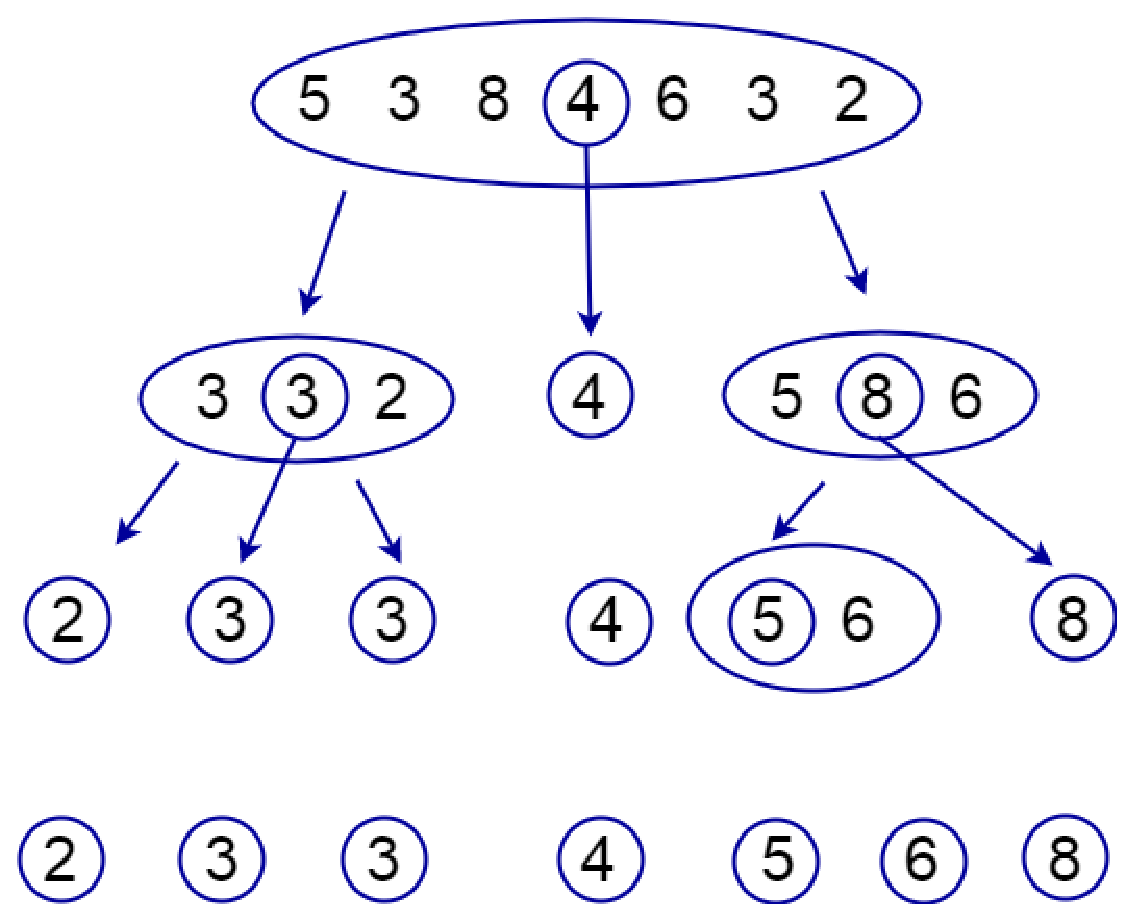
\includegraphics{obr/image.eps}}
	\end{center}
\end{frame}
%%%%%%%%%%%%%%%%%%%%%%%%%%%%%%%%%
\begin{frame}
\frametitle{Pseudokód}
	Samotný kód se pak skládá ze dvou částí:
	\begin{itemize}
	\item Hlavní část, která má na starosti dělení na 2 části.
	\item Partion pak přehazuje prvky v závisloti na pivotu.
	\end{itemize}
	
\end{frame}
%%%%%%%%%%%%%%%%%%%%%%%%%%%%%%%%%
\begin{frame}[fragile]
	\begin{lstlisting}[language=VHDL]
	
quicksort(A, lo, hi) is
    if lo < hi then
        p := partition(A, lo, hi)
        quicksort(A, lo, p - 1)
        quicksort(A, p + 1, hi)

partition(A, lo, hi) is
    	pivot := A[hi]
    	i := lo
    	for j := lo to hi - 1 do
        	if A[j] < pivot then
            	swap A[i] with A[j]
            	i := i + 1
    	swap A[i] with A[hi]
    	return i
       
	\end{lstlisting}
\end{frame}
%%%%%%%%%%%%%%%%%%%%%%%%%%%%%%%%%
\begin{frame}
	\frametitle{Rychlost algoritmu}
	Výkonnost quicksortu je dána volbou pivota. 
	
	Pokud jej volíme ideálně, tak dojde při každém rekurzívním volání k rozpůlení pole a 	vystačíme si tedy s $log_{2}{n}$ voláními, v nichž popřehazujeme až n prvků. 				Složitost tohoto případu je proto $(n \cdot \log_{2}{n})$.
	
	Na druhou stranu, pokud nemáme štěstí a pivota volíme špatně, může se časová náročnost vyšplhat až k $n^2$ \cite{popis}.
\end{frame}
%%%%%%%%%%%%%%%%%%%%%%%%%%%%%%%%%
\begin{frame}
	\frametitle{Volba pivota}
	\begin{itemize}
	 \item První prvek -- popřípadě kterákoli jiná fixní pozice - velice nevýhodná pro byť jen částečně seřazené posloupnosti.
	 \item Náhodný prvek -- často používaná metoda.
	 \item Median -- ideální případ. V praxi to ovšem vždy neplatí, protože výpočet mediánu může být při řazení různých struktur různě náročný a celý algoritmus se jeho výpočtem může zpomalovat. 
	 \item Metoda mediánu tří -- případně pěti či sedmi,... Pomocí pseudonáhodného algoritmu (používají se i fixní pozice, typicky první, prostřední a poslední) se vybere několik prvků z řazené posloupnosti, ze kterých se použitím některého primitivního řadicího algoritmu najde medián a ten je zvolen za pivot.\cite{cvut}
	\end{itemize}
\end{frame}
%%%%%%%%%%%%%%%%%%%%%%%%%%%%%%%%%
\begin{frame}
	\begin{center}
	\renewcommand{\refname}{Použitá literatura}
	\refname
	\bibliography{cit}
	\end{center}
\end{frame}

\end{document}